\addtocontents{toc}{\protect\setlength{\cftsecnumwidth}{13mm}}


\chapter{Diseño}
A continuación, se describe cada caso de uso del PFG siguiendo el orden establecido en el Mapeo de Requerimientos – Casos de Uso. Posteriormente, para agregar valor a la documentación del software, se incluye un diagrama de despliegue, un diagrama de paquetes y un diagrama de estados.  
\section{Gestionar Lugar}

\begin{table}[H]
    \begin{tabular}{@{} *5l @{}} \toprule
    \textbf{Caso de Uso} & Gestionar Lugar \\ \midrule
    Actor & Gerente \\ 
    Descripción & El gerente gestiona un lugar. \\ 
    Propósito & El gerente quiere gestionar un lugar. \\ \midrule
    Precondiciones & El gerente inicia su navegador web. \\ \midrule
    Postcondiciones & Existe un lugar. \\ \midrule
    \multirow{4}{*}{Curso Básico}
        & \parbox{0.75\linewidth}{ 
                1. El gerente visita la página de Lugares. \\
                2. El gerente hace click en el botón Nuevo. \\
                3. El sistema muestra la pagina del formulario de lugar. \\
                4. El gerente ingresa la información correspondiente y envía los datos haciendo click en el botón Guardar. \\
                5. El sistema registra el lugar.  \\
                6. El sistema muestra la página de Lugares.   
        } \\ \midrule
        \multirow{2}{*}{Excepciones}
        & \parbox{0.75\linewidth}{ 
            1. El sistema no puede registrar el lugar dada una falla en la base de datos. \\
            2. El gerente puede salir de la página del formulario de lugar en cualquier momento antes de eliminar haciendo click en Cancelar.
        }  \\  \bottomrule
     \hline
    \end{tabular}
        \caption{Gestionar Lugar - Caso de Uso (1)}
        \label{tab:tabcu-lugar}
\end{table}


\begin{table}[H]
    \begin{tabular}{@{} *5l @{}} \toprule
    \textbf{Caso de Uso} & Gestionar Lugar \\ \midrule
    Actor & Gerente \\ 
    Descripción & El gerente gestiona un lugar. \\ 
    Propósito & El gerente quiere gestionar un lugar. \\ \midrule
    Precondiciones & El gerente inicia su navegador web. Existe el lugar. \\ \midrule
    Postcondiciones & Existe un lugar con nuevos datos. \\ \midrule
    \multirow{4}{*}{Curso Básico}
        & \parbox{0.75\linewidth}{ 
                1. El gerente visita la página de Lugares. \\
                2. El gerente hace click en el boton Modificar de un lugar. \\
                3. El sistema muestra la pagina del formulario de lugar. \\
                    3.1 El sistema recuperara datos del lugar para intentar poblar el formulario. \\
                4. El gerente ingresa la información correspondiente y envía los datos haciendo click en el botón Guardar. \\
                5. El sistema actualiza el lugar.  \\
                6. El sistema muestra la página de Lugares.   
        } \\ \midrule
        \multirow{2}{*}{Excepciones}
        & \parbox{0.75\linewidth}{ 
            1. El sistema no puede actualizar el lugar dada una falla en la base de datos. \\
            2. El gerente puede salir de la página del formulario de lugar en cualquier momento antes de eliminar haciendo click en Cancelar.
        }  \\  \bottomrule
     \hline
    \end{tabular}
        \caption{Gestionar Lugar - Caso de Uso (2)}
        \label{tab:tabcu-lugar}
\end{table}


\begin{table}[H]
    \begin{tabular}{@{} *5l @{}} \toprule
    \textbf{Caso de Uso} & Gestionar Lugar \\ \midrule
    Actor & Gerente \\ 
    Descripción & El gerente gestiona un lugar. \\ 
    Propósito & El gerente quiere gestionar un lugar. \\ \midrule
    Precondiciones & El gerente inicia su navegador web. Existe el lugar.\\ \midrule
    Postcondiciones & Se eliminó un lugar. \\ \midrule
    \multirow{4}{*}{Curso Básico}
        & \parbox{0.75\linewidth}{ 
                1. El gerente visita la página de Lugares. \\
                2. El gerente hace click en el botón Detalles de un Lugar. \\
                3. El sistema muestra la pagina de Detalles de un Lugar. \\
                    3.1 El sistema recupera datos del Lugar para mostrar los detalles. \\
                4. El gerente elimina el lugar haciendo click en el botón Eliminar. \\
                5. El sistema elimina el lugar.  \\
                6. El sistema muestra la página de Lugares.   
        } \\ \midrule
        \multirow{2}{*}{Excepciones}
        & \parbox{0.75\linewidth}{ 
            1. El sistema no puede eliminar el lugar dada una falla en la base de datos. \\
            2. El gerente puede salir de la página de detalles en cualquier momento antes de eliminar haciendo click en Cancelar.
        }  \\  \bottomrule
     \hline
    \end{tabular}
        \caption{Gestionar Lugar - Caso de Uso (3)}
        \label{tab:tabcu-lugar}
\end{table}
    
    
    \begin{figure}[H]
        \centering
        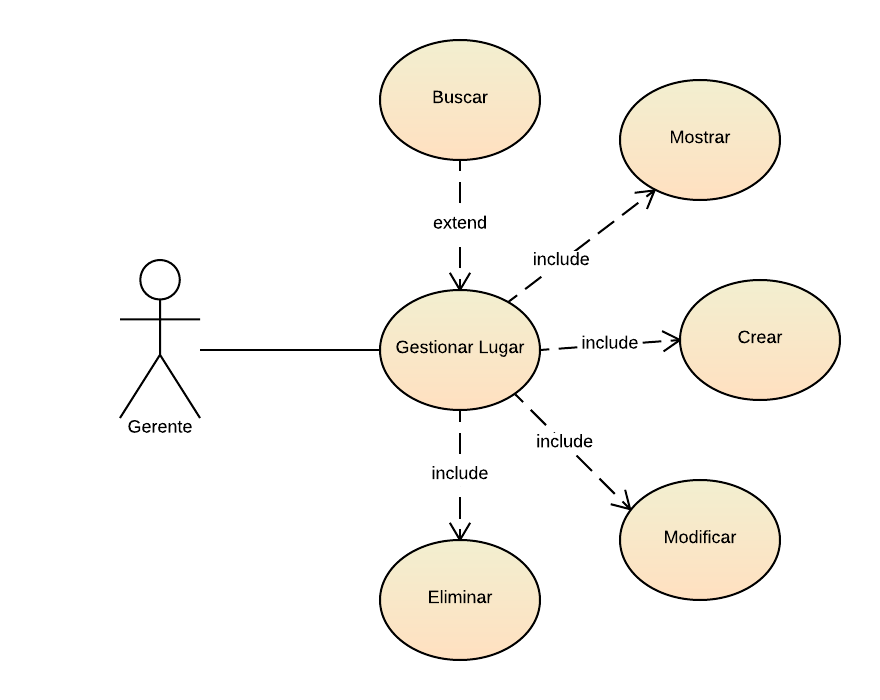
\includegraphics[width=0.85\textwidth]{chapter10/lugar-uc}
        \caption{Gestionar Lugar - Diagrama de Caso de Uso}
        \label{fig:lugar-uc}
    \end{figure}
    
    \begin{figure}[H]
        \centering
        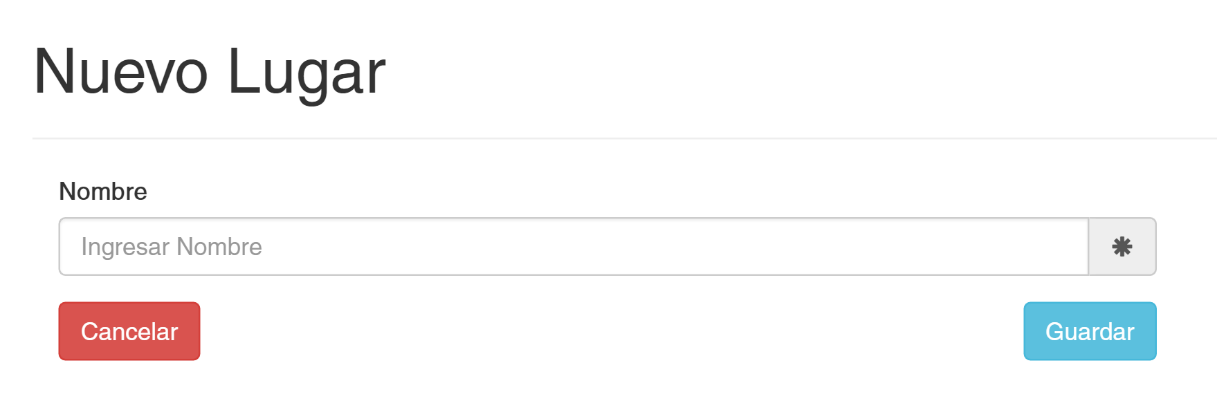
\includegraphics[width=1\textwidth]{chapter10/lugar-int}
        \caption{Gestionar Lugar - Interfaz Tentativa }
        \label{fig:lugar-int}
    \end{figure}
    
    \begin{figure}[H]
        \centering
        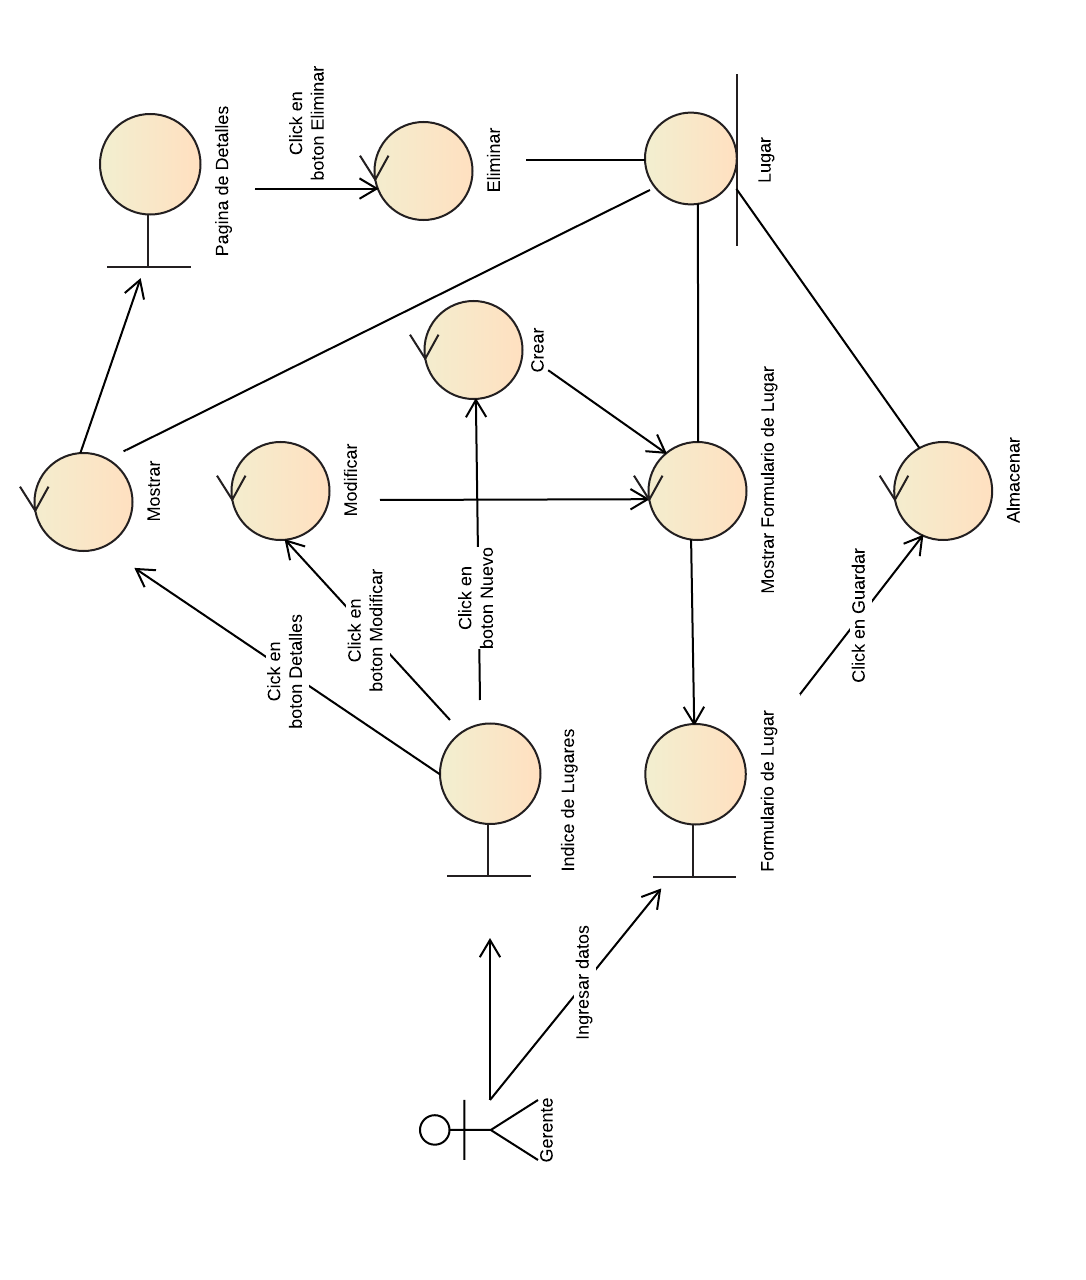
\includegraphics[width=1\textwidth]{chapter10/lugar-rob}
        \caption{Gestionar Lugar - Diagrama de Robustez}
        \label{fig:lugar-rob}
    \end{figure}
    
    \begin{figure}[H]
        \centering
        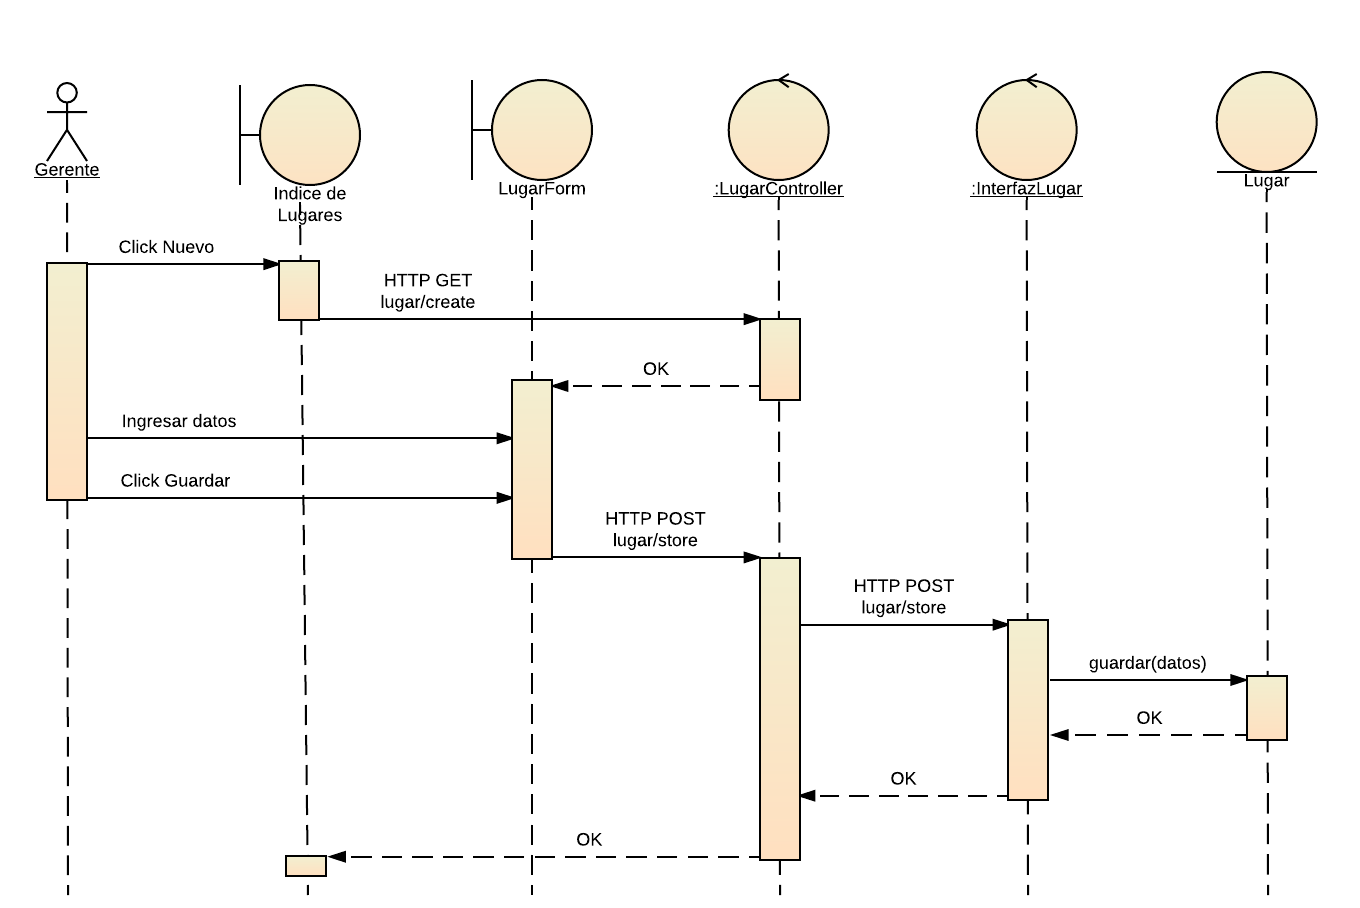
\includegraphics[width=.8\textwidth]{chapter10/lugar-seq-create}
        \caption{Gestionar Lugar - Diagrama de Secuencia (1) }
        \label{fig:lugar-seq-create}
    \end{figure}
    
    \begin{figure}[H]
        \centering
        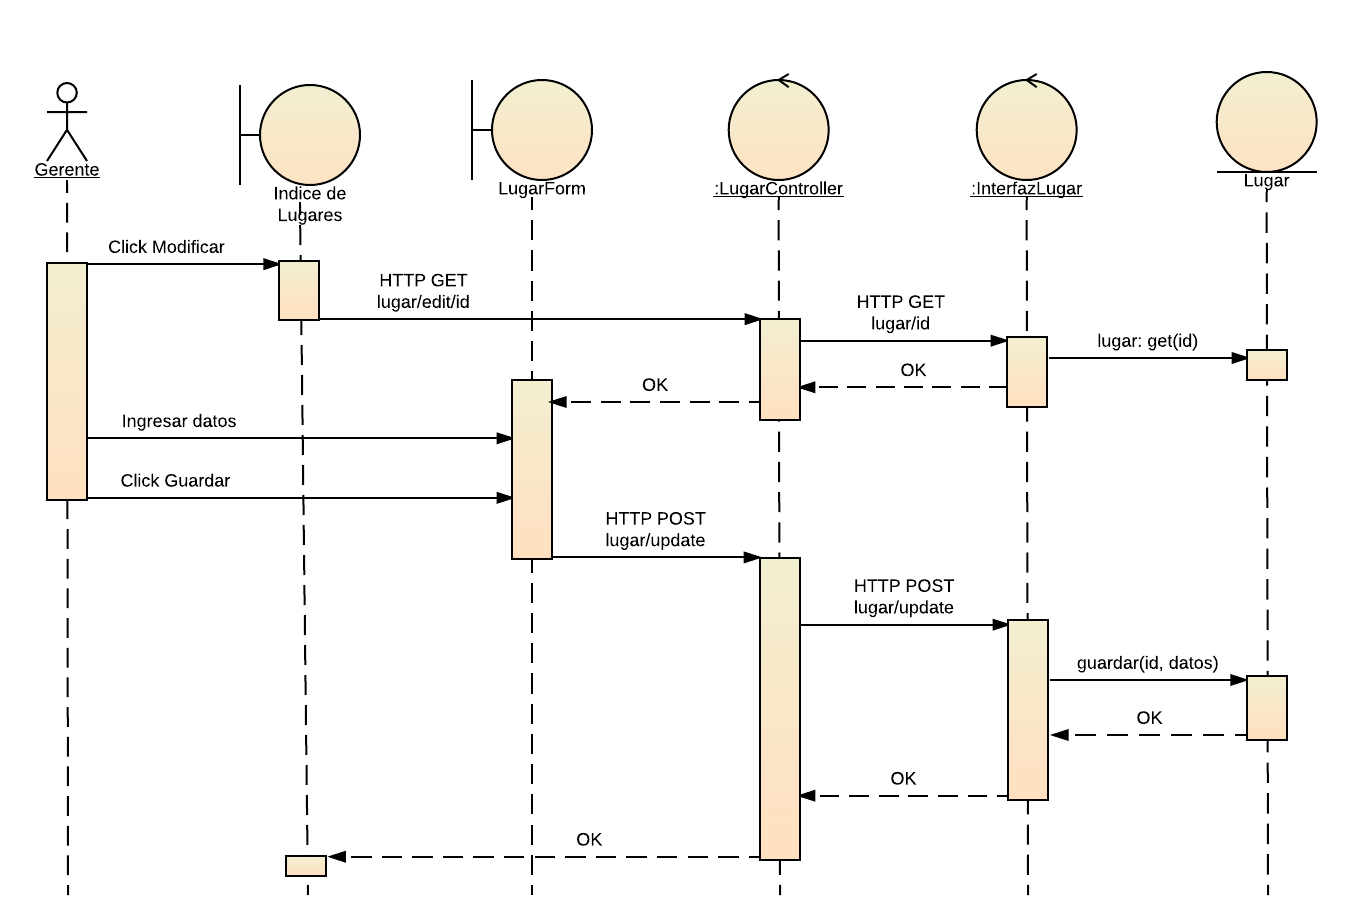
\includegraphics[width=.8\textwidth]{chapter10/lugar-seq-edit}
        \caption{Gestionar Lugar - Diagrama de Secuencia (2) }
        \label{fig:lugar-seq-edit}
    \end{figure}
    
    \begin{figure}[H]
        \centering
        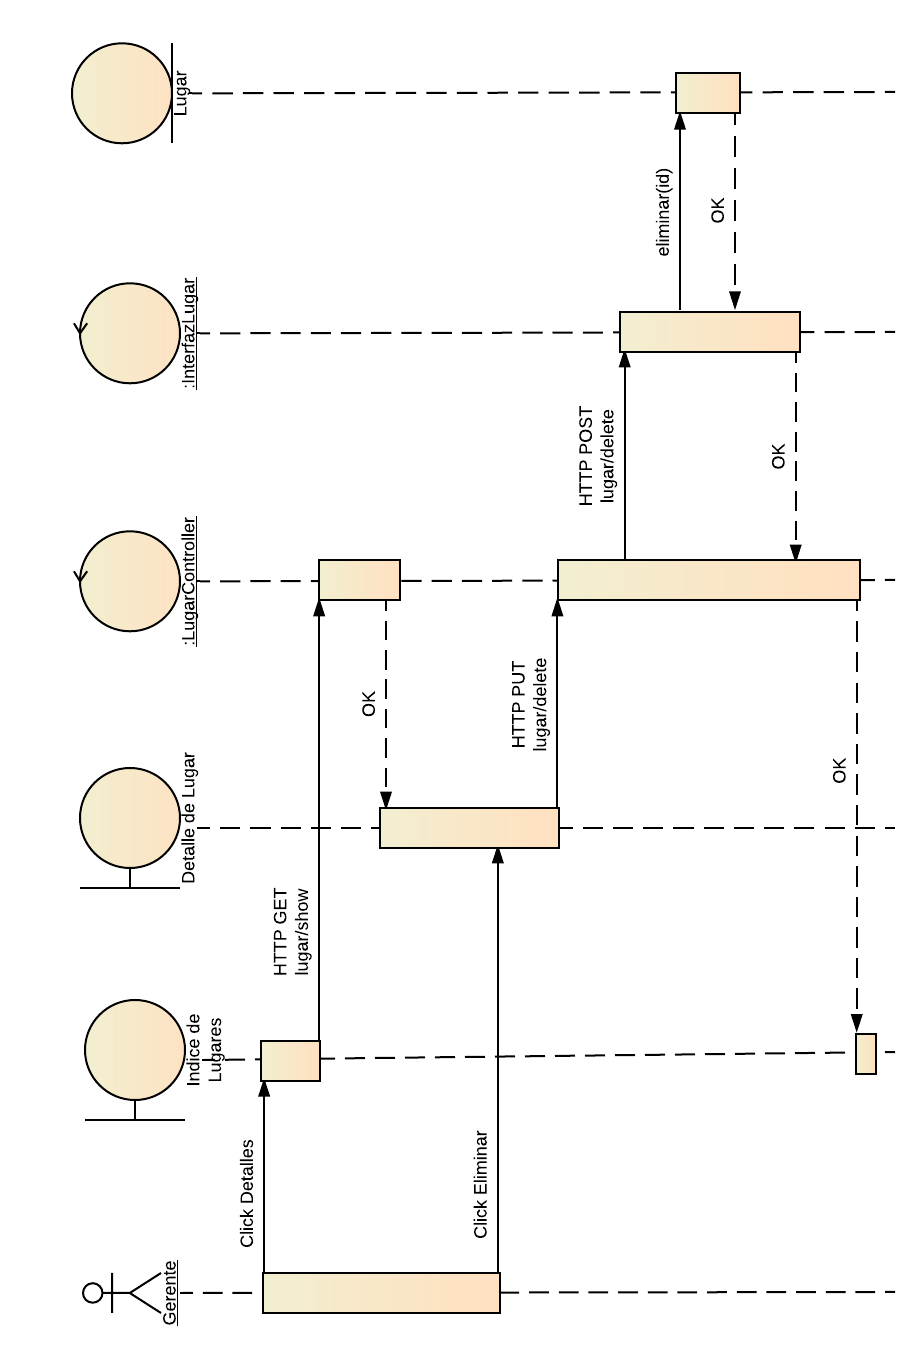
\includegraphics[width=.8\textwidth]{chapter10/lugar-seq-del}
        \caption{Gestionar Lugar - Diagrama de Secuencia (3) }
        \label{fig:lugar-seq-del}
    \end{figure}

\section{Gestionar Cámara}
a
\section{Gestionar Matricula}
a
\section{Gestionar Propietario}
a
\section{Gestionar Coincidencia}
a
\section{Gestionar Recolección}
a
\section{Gestionar Reconocimiento}
a
\section{Gestionar Reporte}
a

\section{Diagrama de Despliegue}
a
\section{Diagrama de Paquetes}
\section{Diagrama de Estados Reconocimiento}

\addtocontents{toc}{\protect\setlength{\cftsecnumwidth}{10mm}}